\chapter{General introduction}
\label{ch:chapter01}
\clearpage{\thispagestyle{empty}\cleardoublepage}

\section{Overview}
The work presented in this thesis can be understood by tracing two major lines of research. The first research line attempts to elucidate the neural correlates of conscious perception, in particular the contents of visual consciousness in humans. The second line concerns human neuroimaging using (functional) magnetic resonance imaging (f/MRI), specifically the new opportunities and challenges that come with moving to ultra-high magnetic field (UHF; 7 Tesla [T] and above). The aim of the present chapter is to provide background on each of the two research paradigms and to motivate the current work at their intersection.

As pointed out by the philosopher of science Imre Lakatos \parencite*{Lakatos1970} every research program can be characterized by a "hard core" and a "protective belt". The hard core is constituted by a sequence of central theses and theoretical assumptions. In order to be able to subject this theory to empirical tests, every research program also has its protective belt of auxiliary hypotheses surrounding the hard core. Researchers spend much of their time on issues related to the protective belt. Therefore, next to tracing the main tenets of the two research programs that underlie the current work, the auxiliary equipment that was necessary to perform the research presented here will also be highlighted. This includes the tools that were needed to work within the two paradigms.

A note on style in the beginning. As is common in contemporary science, a large part of the work presented in this thesis represents a group effort. For this reason, in all empirical chapters the first person plural ("we") will be used. For the Introduction and General Discussion section, some sections contain personal memories or opinions. In these exceptional cases, the first person singular ("I") will be used.

\section{Neural correlates of consciousness}
The work presented here is motivated by the question of how human conscious experience relates to cortical activity in our brains. As such, the work is part of a larger research paradigm that aims to identify the neural correlates of consciousness (NCC). To better understand the aim of this paradigm, it is helpful to first clarify what is meant by the term "neural correlate of consciousness". The philosopher of mind David Chalmers \parencite*{Chalmers2000} offered the following, approximative definition:

\begin{quotation}
"A neural system N is an NCC if the state of N correlates directly with states of consciousness." \parencite[p. 3]{Chalmers2000}
\end{quotation}

Taking this definition as a starting point, he then elaborated on two aspects: what the relevant "states of consciousness" are and what it means for a neural state to "correlate directly" with states of consciousness. The focus here is on the states of consciousness, since the sense in which correlation will be used throughout this thesis is equivalent to the scientific notion of correlation - i.e. correlation as operationalized by Pearson's correlation coefficient.

Chalmers \parencite*{Chalmers2000} distinguished three broad classes of conscious states. The first class is binary and the conscious states belonging to that class are those of being conscious and of not being conscious. The second class concerns background states of consciousness such as being asleep, being awake, dreaming or being under hypnosis \parencite{Chalmers2000}. Although the neural systems correlating with states in these two classes are crucial to human everyday functioning (as we are reminded of in critical clinical conditions such as coma or death), they are not the subject of the current work.

\subsection{Content-specific NCC}
Instead, the focus of this thesis and "arguably the most interesting states of consciousness" \parencite[p. 4]{Chalmers2000} are the states of subjective experience that humans are in at any given moment in time. This third class is called the contents of consciousness because states in this class are distinguished by their specific representational content. Example states for this class are the experience of a particular sound pattern or the experience of a visual scene. What characterizes these states is that they represent the world to be one way or another. The experience of a visual scene, for example, represents the world to contain particular arrangements of objects with particular shapes and particular spatial relationships to one another. This does not mean the experience needs to be veridical. During hallucination or when experiencing the visual illusions used in this thesis, for example, the world is not the way that the experience represents it as being. What matters is that all conscious states in this class have distinct representational content.

The search for the neural correlates of the contents of consciousness (in brief, content-specific NCC; \cite{Koch2016}) usually proceeds in two steps (see Figure~\ref{fig:ncc}). First, in a mapping step, researchers determine the receptive field (RF) of a recording site (either a neuron in single-cell electro-physiology studies or a voxel in fMRI studies). This involves determining the selectivity profile of a recording site in response to the variation of a specific parameter. This parameter will differ depending on the aspect of a conscious experience that a researcher is interested in. The parameter could, for example, be the orientation of a stimulus, its motion direction, its position, etc. For the study described in Chapter 3, the parameter of interest was visual motion axis and during the mapping step we determined whether voxels were selective to horizontal or vertical motion. Importantly, during the mapping step, stimuli are presented in an unambiguous manner, meaning that, for awake and healthy human adults, there is only a single perceptual interpretation of the stimulus.

\begin{figure}[!htbp]
\centering
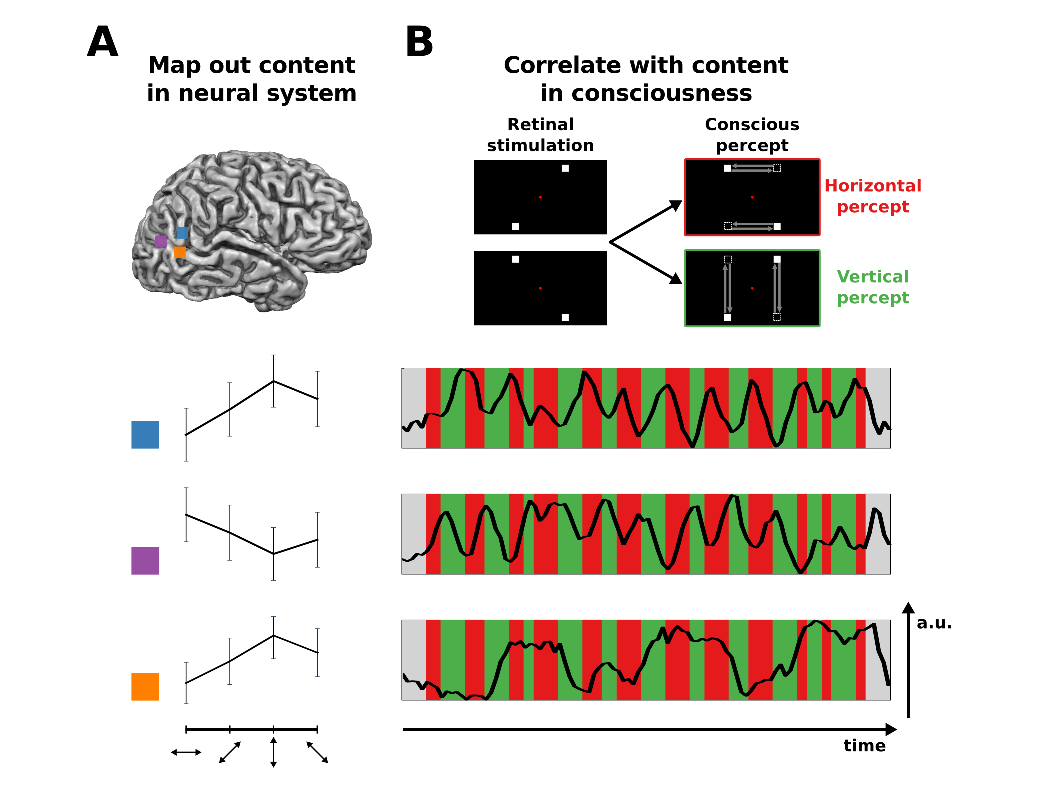
\includegraphics[width=\textwidth]{figures/chapter_01/fig1.eps}
\caption{Approach for identifying neural correlates of the contents of consciousness. \textbf{(A)} In a first mapping step researchers determine the receptive field of a recording site. In this example, the selectivity profile of three different voxels (blue, purple and orange) is determined in response to different axes of visual motion. Axis-of-motion stimuli are presented in an unambiguous manner along four clearly determined motion axes (horizontal, vertical and two oblique axes). \textbf{(B)} In a second step subjects are exposed to an ambiguous stimulus. In this example, the bistable motion quartet can give rise to the conscious percept of either horizontal (red) or vertical (green) motion although the retinal stimulation remains constant over time. While participants communicate their conscious percept at any given moment in time  (shown as distinct perceptual periods in red or green), the researcher monitors activity in the recordings site (shown as black time series for each of the three voxels). This procedure allows the researcher to track the representational content in the neural system of interest and to see if it matches the content in the subject's consciousness. The blue voxel, for example, appears to be selective to vertical motion and also shows increased signal when the subject indicates perceiving vertical motion (the same applies to the purple voxel for horizontal motion), while the orange voxel shows a preference for vertical motion in the first step but does not modulate its signal with the conscious percept in the second step. a.u. stands for arbitrary unit.}
\label{fig:ncc} 
\end{figure}

In a second step, subjects are exposed to an ambiguous stimulus (setup) that allows for more than one perceptual interpretation. Typical methods for achieving perceptual ambiguity in visual neuroscience are multistable figures, binocular rivalry or continuous flash suppression. The underlying idea is the same: while the physical stimulus properties remain constant, the contents of consciousness alternate over time between different interpretations of the stimulus. For example, for the study described in Chapter 3 we presented participants with the bistable motion quartet \parencite{Ramachandran1985} which yields alternating conscious experiences of either horizontal or vertical motion although the retinal stimulation remains constant (see Figure~\ref{fig:ncc}). Participants communicate what they are experiencing at any given moment in time, which is usually achieved via corresponding button presses, while the researcher monitors the concurrent responses in recording sites whose RFs were mapped in the first step.

This procedure allows the researcher to track the representational content in the neural system of interest and to see if it matches the content of the subject's experience. If a recording site has been identified, for example, as preferring horizontal motion in the first step and shows responses that systematically correlate with the subject indicating the experience of horizontal motion in the second step, then it should be considered (part of) the content-specific NCC for horizontal motion experience.

Compared to the first two classes of conscious states, the search for content-specific NCC thus poses an extra requirement on the NCC. It requires that the representational content of the neural state in question matches the content of the conscious state. The additional requirement yields increased explanatory and predictive power because once a content-specific NCC has been identified it can be used to predict the presence or absence of phenomenal features in conscious experience based on the neural state of the system \parencite{Chalmers2000}. The definition of a content-specific NCC can be updated to capture this additional requirement:

\begin{quotation}
"A neural correlate of the contents of consciousness is a neural representational system N such that representation of a content in N directly correlates with representation of that content in consciousness." \parencite[p. 6]{Chalmers2000}
\end{quotation}

\subsection{Chalmer's caveat: content-specific NCC in humans}
This definition has an important implication for the search of content-specific NCC. It is crucial that the researcher is able to map out the RF of a recording site so s/he can track the representational content in a neural system by tracking its activity. Twenty years ago, when David Chalmers laid out the NCC definitions above, he noted that, given this requirement, in practice

\begin{quotation}
"...the most informative and useful results usually come from neuron-level studies on monkeys. Large claims are sometimes made for brain imaging on humans, but it is generally difficult to draw solid conclusions from such studies, especially where an NCC is concerned. We can trace the difference to the fact that neuron-level studies can monitor representational content in neural systems, whereas imaging studies cannot (or at least usually do not)."
\parencite[p. 25]{Chalmers2000}
\end{quotation}

This verdict, which I will refer to as "Chalmer's caveat" below, has been damning for fMRI research into the NCC and might explain why many researchers in the consciousness community show a fair amount of skepticism towards brain imaging methods like fMRI. I remember joining my first meeting of the Association for the Scientific Study of Consciousness (ASSC) in 2014, which took place in Brisbane, Australia. The conference committee organized a mentor lunch where young researchers had the opportunity to receive career advice from researchers that were already established in the field. In this context, I had the pleasure of meeting Sid Kouider \parencite{Kouider2010}, a respected consciousness researcher from the École Normale Supérieure in Paris. Reflecting the general turn of the consciousness community away from fMRI and towards conceptual issues and psychophysical studies, Sid Kouider did not see much potential in fMRI research for studying consciousness ("with the exception of MVPA studies"). I believe he summarized the overall sentiment of the community accurately; at least during the ASSC conference in Paris in the subsequent year, among hundreds of contributions on consciousness the keyword "fMRI" appeared only twice in the conference proceedings - one of which resulting from our own work.

However, I did not follow Sid Kouider's advice and I believe in several ways the current work is testimony to the progress in human neuroimaging that has taken place since. Although it is still not possible to monitor the activity of single neurons in humans non-invasively, I would submit that Chalmer's caveat for human brain imaging methods is no longer applicable to fMRI. Progress in MRI technology \parencite{Vaughan2001, Duyn2011, Ugurbil2014} and fMRI analysis techniques \parencite{Wandell2015, DeMartino2016, Kashyap2017, Kemper2017, Polimeni2017} have developed fMRI into a tool that allows researchers to monitor the representational content also in human brain systems. On the MRI technology side, the work presented here has in particular benefited from the development of UHF MRI scanners for neuroimaging in humans \parencite{Ugurbil2003}. With regard to fMRI analysis, two techniques were particularly crucial in the context of this thesis. One is the ability to distinguish and record from distinct (columnar) clusters within human cortex \parencite{Cheng2001, Yacoub2007, Yacoub2008}, which was used in Chapter 3. The other one is population RF (pRF) mapping \parencite{Dumoulin2008}, which allows to define the RF properties of single voxels in human fMRI studies and was used in Chapter 4. These methodological advances are reviewed below after briefly highlighting why studying content-specific NCC in human, as opposed to non-human, subjects is important.

\subsection{Why we should study NCC in humans}
Studying conscious states in humans directly has obvious advantages. I remember vividly the comments that I received when writing an educational piece on the search for the NCC that was aimed at the general public. To familiarize readers with the research program, I summarized and described classic experiments using binocular rivalry in primates \parencite{Logothetis1989, Sheinberg1997}. The comments from the general public reflected some skepticism towards the research agenda; one comment in particular ridiculed the approach: "Haha, they are trying to study consciousness ... in MONKEYS!!!" Admittedly, this comment unduly inflates the difference between human and non-human primates and, in my opinion, we should expect humans and other primates to share fundamental aspects of their conscious experience.

However, I think the comment also points to at least two important aspects. First, compared to studies on monkeys, human neuroimaging studies have the advantage that evidence for conscious content can be gathered more straightforwardly. Monkeys require additional training to learn to communicate their conscious percept. Even once monkeys have learned to press the "corresponding" buttons, drawing conclusions about human consciousness from monkey research will always require the additional assumption that monkeys perceive visual illusions in a way similar to us. Admittedly, the privacy of conscious experience combined with the problem of other minds require researchers to make similar assumptions for human subjects. Yet this effort is facilitated by the human ability to use verbal report to describe what they experience. Second, although we should expect many similarities in (content-specific) NCCs between human and non-human primates, owing to vast commonalities in brain anatomy and function, there might also be important differences - especially since the studied primates were macaque monkeys which are phylogenetically more distant from humans than great apes such as chimpanzees or bonobos. These differences can only be explored if appropriate human brain imaging studies are conducted.

\section{Neuroimaging at uhf: new opportunities}
\subsection{Higher field strength, more sensitivity}
Moving to UHF MRI confers specific advantages and disadvantages to fMRI studies of the human brain. The most prominent advantage of UHF, as compared to conventional field strengths (such as 1.5, 3 and 4 T), is an increase in sensitivity. It is not straightforward to determine by how much exactly signal-to-noise ratio (SNR) increases with additional field strengths since, at UHF, SNR is a complex function of resonance frequency (and thus static magnetic field strength [B0]) but also of head size, head shape, position within the head and tissue composition \parencite{Ugurbil2003}. Most derivations suggest at least linear increases in SNR above 3 T \parencite{Ladd2018} and the power factor x in $B0^x$ for maximum theoretically achievable SNR is estimated to be between 1.2 and 2.1, depending on whether a voxel is at the surface or deep inside the brain \parencite{Ladd2018}.

The increase in sensitivity can be leveraged in several ways. It can be used to reduce scan time, to include more experimental conditions or to enable single-subject studies that were starved for SNR at conventional field strengths \parencite{Polimeni2017}. The most common use, however, is to trade the gain in SNR for an increase in spatial or temporal resolution \parencite{Polimeni2017}. This provides new opportunities and, as many have argued, offers new classes of experiments (for reviews, see \cite{Polimeni2017, DeMartino2016, Dumoulin2017}). Here, the focus will be on applications that have used the additional SNR from UHF to offset (some of) the SNR that is lost when moving to very high spatial resolution. This is desirable for at least two reasons. First, it allows researchers to translate SNR gains at UHF to tSNR more efficiently. Second, it enables researchers to study how functional properties change within the cortical ribbon, along surfaces and across cortical depths. The following sections will elaborate on these two aspects in turn.

\subsection{Higher SNR translates to tSNR at high-resolution}
One motivation to move to higher resolutions is to use the gains in image SNR efficiently. Temporal SNR (tSNR), which is directly related to statistical power in e.g. univariate analyses, is a linear function of image SNR \textit{only if} no physiological fluctuations exist \parencite{Murphy2007}. In the presence of physiological noise tSNR plateaus when a particular level of SNR is reached. However, when moving from conventional to high spatial resolutions the noise regime switches from being dominated by physiological modulations to being dominated by thermal image noise \parencite{Triantafyllou2005}. This shifts the point where tSNR plateaus to higher levels. It was, for example, demonstrated empirically that, for 7T fMRI, SNR gains translated to corresponding tSNR gains at higher resolution (e.g. 1 x 1 x 3 $mm^3$) while only moderate tSNR gains were observed at conventional resolution (e.g. 3 x 3 x 3 $mm^3$) where tSNR was limited by physiological noise \parencite{Triantafyllou2005}. Thus, choosing the spatial resolution appropriately can help to efficiently translate image SNR to temporal SNR at UHF.

\subsection{Neuroimaging at the mesoscale}
The second motivation to move to high resolutions (in the sub-millimeter range) is that it enables researchers to target a new organizational scale of human brain function. The organization of the human brain, and of cortex more specifically, is often divided into three different scales - the microscopic (the level of single neurons), the mesoscopic (the level of neuronal circuits) and the macroscopic scale (the level of brain areas). Until recently, non-invasive human neuroimaging with fMRI was confined to the macroscopic scale allowing researchers to identify and study responses from different brain areas and large-scale brain networks. The increase to sub-millimeter resolution afforded by UHF allows for fMRI investigations to move to the mesoscopic scale. This is important for a number of reasons. For a start, it offers the novel possibility to non-invasively study responses at the level of cortical columns, cortical layers, and subcortical nuclei. fMRI research at the mesoscale thus promises a plethora of new empirical insights. Furthermore, some scientists assign particular meaning to the mesoscale in cognitive and computational neuroscience research since they believe that (some) mesoscopic structures might represent fundamental units of neural computations \parencite{Hubel1974, Dumoulin2017}. Accordingly, one key to understanding brain function is to identify these fundamental units and to study their responses. More conservatively, the mesoscopic scale is a relevant organisational level since it represents an intermediate level of analysis where information from individual neurons and brain areas meet \parencite{Mitra2014, DeMartino2016}. At the very least, sub-millimeter fMRI studies might help to bridge the gap between theories of cognitive computation, which are usually formulated at the microscopic or mesoscopic level, and empirical studies in humans, which were hitherto conducted at the macroscopic scale \parencite{MarquardtPhDThesis}.

\subsection{Mapping cortical columnar structures}
Sub-millimeter cortical fMRI studies can be divided into so-called "laminar" studies that investigate fMRI responses as a function of cortical depth and "columnar" studies that functionally map columnar structures - i.e. structures that share a singular feature in the cortical depth direction. It is important to note that the meaning of the terms "laminar" and "columnar" in the fMRI community differs from that in cellular and molecular neuroscience. Even at the very high spatial resolutions now achievable with fMRI (0.7 or 0.8 mm isotropic), it is not possible to resolve signal from distinct histological layers or microcolumns. To highlight the difference from histology, laminar fMRI studies are alternatively referred to as "cortical-depth dependent" fMRI. For columnar fMRI there is currently no established alternative although the suffix "-like" (as in "columnar-like") is often employed. Problematically, even within fundamental neuroscience, there are different meanings to the term "column" resulting from differences in the defining feature (function, cell constellation, connectivity or myelin content), the extent of columns, and their spatial organization \parencite{Rakic2008}. We have recently proposed the term "columnar clusters" to refer to functionally relevant clusters in reach of high-resolution fMRI \parencite{Schneider2019} and this term or the term "columnar-like" will be used throughout this thesis to avoid confusion with histological definitions.

These conceptual issues should not distract from the technological strikes that now enable researchers to record responses in living human beings from different cortical depth levels (such as deep, mid, and superficial levels) or from distinct cortical clusters within the same brain area. While several studies have used UHF fMRI to investigate laminar differences with fMRI \parencite{Ress2007, Polimeni2010, Koopmans2010, Koopmans2011, Olman2012, DeMartino2013, Huber2015, Muckli2015, Kok2016, Huber2017, Marquardt2018, Kashyap2018}, the focus here is on columnar studies. The first fMRI studies to identify columnar-like structures in humans were confined to primary visual cortex (V1) \parencite{Cheng2001, Yacoub2007, Yacoub2008}. This offered important simplifications. First, the ocular dominance and orientation columns in V1 were already well-established by animal electro-physiology \parencite{Hubel1974} and post-mortem histology. Second, these structures were relatively large. Third, in most human individuals V1 is relatively flat, simplifying the recording of signal at different cortical depths and enabling the acquisition even with sequences that have minimal coverage in the slice direction (even with a single slice, \cite{Yacoub2008}). Leaving striate cortex required the development of accurate sampling techniques to deal with the folded cortex in humans \parencite{Polimeni2017, Kemper2017}. Subsequently, researchers identified columnar clusters in human V2, V3, V4 \parencite{Nasr2016, Tootell2017}, V3a \parencite{Goncalves2015} and V5 \parencite{Zimmermann2011} as well as in A1 \parencite{DeMartino2015}.

All these studies used unambiguous sensory stimuli (first step in the NCC approach) but did \textit{not} present ambiguous stimuli that allowed for dissociating neural signals pertaining to conscious perception from those related to sensory stimulation (second step in the NCC approach). Yet the ability to map distinct cortical clusters opens up an important avenue for the search of content-specific NCC. Since each cluster is characterized by a shared preference for a specific feature (e.g. a stimulus orientation, a motion direction, etc.) researchers can now monitor the representational content of columnar systems. Mapping out functional cortical clusters and measuring their responses during ambiguous sensory stimulation thus fulfills the criteria for the search for content-specific NCC outlined by Chalmers \parencite*{Chalmers2000} about 20 years ago and is now feasible in humans with UHF fMRI.

\subsection{More specificity at UHF}
Next to the increase in sensitivity, fMRI also benefits from greater specificity of the blood oxygenation level dependent (BOLD) contrast at UHF. T2 and T2* relaxation times decrease more rapidly for blood than for neuronal tissue when moving to UHF \parencite{Ugurbil2002}. As a consequence, the relative intravascular contribution to the BOLD signal decreases \parencite{Uludag2009, Uludag2016}. This is desirable since intravascular signal partly originates from large ascending cortical and pial veins which are known to show less specific responses than neuronal tissue \parencite{DeMartino2016, Moerel2017}. The shift towards contributions from smaller diameter vessels therefore increases specificity at higher fields. As pointed out by \cite{DeMartino2016}, however, although the extravascular signal around smaller vessels increases more (increase with the square of B0) than signal around larger vessels (approximately linear increase with B0), the signal around larger vessels still increases. Especially for gradient echo (GE) sequences, which have been employed in the studies presented here, signal is therefore still affected by larger, less specific vessels - an issue we will return to in the General Discussion. Next to the increase in BOLD contrast, fMRI at UHF can additionally gain in neuronal specificity if images are acquired at high spatial resolution because partial volume effects are reduced \parencite{DeMartino2016}.

\subsection{Population receptive field modelling}
It is currently not possible to map out RF properties of single neurons in humans using non-invasive neuroimaging methods such as fMRI. However, the introduction of the population RF (pRF) mapping framework \parencite{Dumoulin2008} enables researchers to estimate the spatial RF properties of single voxels in a human fMRI study. The pRF mapping framework is based on the assumption that the neural population that is contained within a voxel has vastly overlapping spatial RF properties. This assumption is reasonable given that spatial RF properties properties are known to vary smoothly along the cortical sheet.

The pRF for a single voxel is determined in a simple procedure. The voxel time course is assumed to be generated by a 2D Gaussian model. This model can be summarized using only three parameters - two parameters to describe the position of the 2D Gaussian in visual space (conventionally called x and y parameters) and one parameter to describe the its size (conventionally called sigma parameter). During the pRF mapping experiment, stimuli are presented that occupy varying positions in visual space (see Figure~\ref{fig:prf}). This can for example be a bar stimulus that, over the course of a pRF mapping run, steps through the visual field. Conventionally, pRF mapping stimuli reveal a checkerboard pattern \parencite{Dumoulin2008}, although alternative carrier patterns have been suggested and used \parencite{Alvarez2015}.

Depending on the specific parameters that are assumed, the convolution of the 2D Gaussian with the spatial apertures of the stimulus presented during the pRF mapping run leads to distinct time series predictions. For example, if a 2D Gaussian is assumed to be centered on the left horizontal meridian several degrees away from fixation, then a bar stimulus stepping through the visual field from left to right should evoke activity in the beginning of the but not in the end of the mapping run. By systematically varying the parameters of the 2D Gaussian and comparing the predicted time series against the measured time series of a voxel, the three pRF parameters can be optimized to accurately summarize the spatial pRF properties of a voxel. To account for hemodynamic delay in the fMRI response, the predicted model time course is usually convolved with a canonical double-gamma function \parencite{Friston1998}.

\begin{figure}[!htb]
\centering
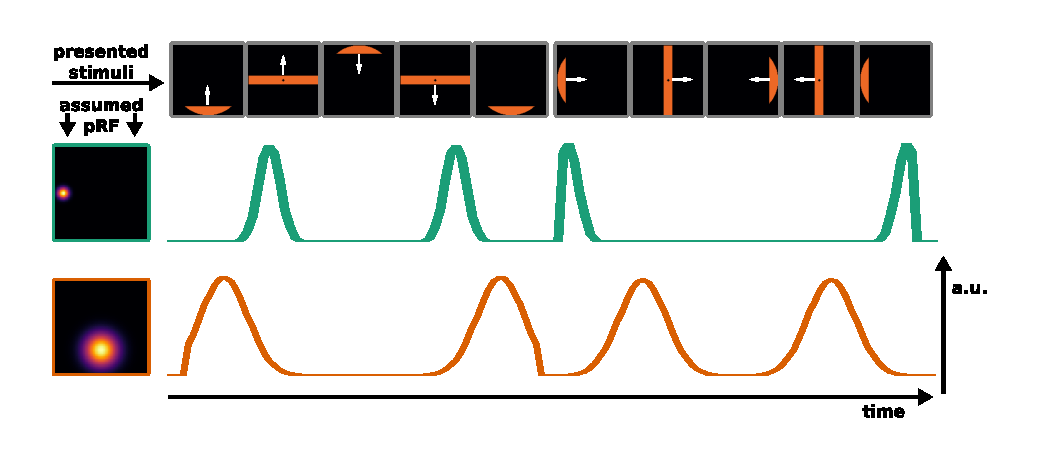
\includegraphics[width=\textwidth]{figures/chapter_01/fig2.eps}
\caption{pRF mapping framework. During the pRF mapping experiment, the position of the stimulus is systematically varied. In this example, a bar first stepped from bottom to top and back and then from left to right and back (exemplary bar positions are shown on top). Depending on the position and size of the assumed pRF, the stimuli evoke a particular response time course. In this example, two exemplary pRFs are assumed (shown on the left, green and orange pRF). The green pRF shows responses only when the bar stimulus crosses the left, central region of the visual field. Due to its larger size, the orange pRF shows broader tuning and shows responses when the bar crosses the central, bottom part of the visual field. a.u. stands for arbitrary unit.}
\label{fig:prf} 
\end{figure}

Since its conception \parencite{Dumoulin2008}, pRF mapping has yielded many exciting insights into the organization of visual field maps in humans \parencite{Amano2009, Winawer2010, Harvey2011, Zuiderbaan2012, Kay2013, Klein2014, Kay2015, Harvey2015, Fracasso2016}. Although it is possible to measure pRFs at lower resolutions and conventional field strengths, pRF mapping benefits from the increase in spatial resolution and neuronal specificity afforded by UHF since the distribution of neurons in terms of their RF becomes more homogeneous \parencite{DeMartino2016}. As a result, pRF estimates will be more specific. This is relevant for studies aiming to measure small changes in pRF properties in response to an experimental manipulation (see Chapter 4) since more specific pRF estimates yield increased power for picking up pRF differences.

Although pRF mapping benefits from higher spatial resolution, this does not necessarily mean that \textit{sub-millimeter} resolution is beneficial in this context. It is sometimes forgotten in the UHF community that there is no imperative obligating researchers to acquire images at mesoscopic resolution when operating UHF scanners. Admittedly, given the considerations about tSNR and partial volume effects outlined above, it is preferable to operate high field scanners at high spatial resolutions. Furthermore, the increase in sensitivity that comes with UHF offsets the loss in SNR incurred by increasing voxel resolution. Consequently, sensitivity is roughly similar between a 2 mm isotropic voxel at 3T and a 1.6 mm isotropic voxel at 7T \parencite{DeMartino2016}. However, increasing resolution even further comes at the expense of sensitivity. Depending on the research question, measuring responses at the sub-millimeter scale might therefore not be desirable. This can be the case for pRF mapping. The increase in specificity for pRF estimates motivates higher resolutions, yet if the research question does not concern laminar or columnar neuronal populations, sub-millimeter resolution unnecessarily sacrifices sensitivity and resolutions between 1.1 and 1.5 mm isotropic might represent a more appropriate choice (see Chapter 4).

\section{Neuroimaging at uhf: new challenges}
Despite the distinct advantages that come with performing fMRI experiments at UHF, there are also several challenges that need to be addressed first to harvest the full potential of UHF fMRI, especially for fMRI studies with sub-millimeter resolution. Here, four methodological problems are highlighted since tackling them was important ground work for the empirical research presented in Chapter 3 and 4. Additional challenges for UHF analyses and their impact on statistical analyses have been discussed and reviewed elsewhere \parencite{Polimeni2017, DeMartino2016}.

\subsection{Wanted: an anatomical reference}
Many of the challenges at UHF are interlinked and relate to building an anatomical reference for the fMRI data \parencite{Polimeni2017}. An anatomical reference is necessary, for example, in order to determine which fMRI responses originate from gray matter, to sample cortical-depth dependent responses (laminar or columnar), or to reconstruct cortical surfaces for delineating specialised cortical areas such as visual field maps. With this aim in mind, next to functional images, researchers usually acquire images that are rich in anatomical contrast. A common choice for this are images from magnetization-prepared T1-weighted pulse sequences (MPRAGE and MP2RAGE) \parencite{Mugler1990, Moortele2009, Marques2010}. These sequences offer good white matter (WM) / gray matter (GM) / cerebrospinal fluid (CSF) contrast and can be recorded at high spatial resolution (0.6 mm isotropic) in less than 15 minutes.

Whether to opt for the MPRAGE or MP2RAGE sequence is mostly a matter of taste; yet there are some considerations that can guide the decision. Both sequences are negatively affected by the non-uniform radiofrequency (RF) transmit field (B1+) at UHF. In the case of MPRAGE, this problem can be addressed by acquiring, next to the T1 weighted (T1W) image, a matched proton-density weighted (PDw) image \parencite{Moortele2009}. Division of the two images normalizes the intensity bias. The MP2RAGE sequence is a modification of the MPRAGE sequence that records two different images at different inversion times and combines them to reduce B1+ bias \parencite{Marques2010}.

These differences in acquisition and reconstruction lead to distinct advantages and disadvantages. Acquisition time for MPRAGE images can be slightly longer than for MP2RAGE images - although the difference is 3-5 minutes at most for sub-millimeter resolution. Most software packages have been bench-marked on T1w MPRAGE images, which might make processing of MPRAGE images easier, although the MP2RAGE sequence also yields a "uni" image that offers similar contrast. Lastly, the MP2RAGE sequence usually yields images with superior WM contrast, while MPRAGE images allow for better delineation of the GM/CSF boundary. This is because division of T1w by PDw images highlights blood vessels \parencite{Moortele2009} which can then be correctly excluded from GM (at least by manual or semi-automatic segmentation methods, see Chapter 2). As a rule of thumb, MPRAGE images can therefore be recommended when high-quality delineations of both WM/GM and GM/CSF boundaries matter (e.g. for columnar fMRI; see Chapter 3) while MP2RAGE should be used if only a good delineation of the WM/GM is required (e.g. for surface reconstruction and display of visual field maps; see Chapter 4).

\subsection{Co-registration}
Once functional and anatomical images have been acquired, one of the first challenges is to co-register them. The same challenge exists with images acquired at conventional field strengths but there are at least two peculiarities that make this task more challenging at UHF. The first is that the functional images will show geometric distortions (see below). The second is that functional images will be acquired even more often with partial coverage only. In such cases, boundary-based registration (BBR) \parencite{Greve2009} can offer satisfactory solutions, provided that the functional images show at least some WM/GM contrast. BBR optimizes the position of the WM/GM surface reconstructed from the anatomical images with respect to the boundary between gray and white matter in the fMRI data. Since BBR thus attempts to match the WM/GM boundaries in anatomical and functional data, it is ideally suited for fMRI analyses that require a very accurate alignment of cortical boundaries \parencite{Polimeni2017} (which was the case for the studies presented in Chapter 3 and 4).

\subsection{Geometric distortions}
Two of the most commonly used sequences for the acquisition of high-resolution functional images are 2D \parencite{Feinberg2010, Moeller2010, Setsompop2012} and 3D \parencite{Poser2010} gradient-echo (GE) echo planar imaging (EPI) sequences (alternatives are reviewed in the General Discussion). The resulting EPI data suffer from larger geometric distortions at UHF meaning that they no longer represent size and shape of the brain accurately. This is problematic since anatomical images obtained from MPRAGE derivatives retain the shape of the brain relatively well and, as a result, functional and anatomical images no longer match. Different solutions exist for this problem, three of which have been reported \parencite{DeMartino2016}. One can record images that are matched in their distortions to the functional images but have sufficient contrast for segmentation of GM \parencite{Renvall2016, Kashyap2017}; one can perform segmentation on functional images directly provided that they have sufficient contrast \parencite{Fracasso2016}; or, one can attempt to correct the distortions in the functional images \parencite{Emmerling2016, Marquardt2018}. All these solutions can be understood as a trade-off between co-registration and segmentation performance. While the first two solutions minimize co-registration error at the expense of segmentation error, the last solution minimizes segmentation error but increases the possibility of mismatches between functional and anatomical images.

\subsection{Registration between sessions}
Although the increase in SNR that comes with imaging at UHF offsets some of the SNR loss that is incurred by moving to very high resolutions, not all of the SNR is necessarily offset. This can be remedied by acquiring more data and by using averaging techniques. If one is interested in single-subject columnar or laminar effects then, depending on the effect size, even for a simple experiment with only two experimental conditions, data from more than one scanning session might be required to have sufficient statistical power (see Chapter 3). Likewise, if the resolution is not sub-millimeter but still high (between 1 to 1.2 mm isotropic) and many different experimental conditions are required, sufficient data for averaging is still crucial (see pRF mapping in Chapter 4).

Combining data from different scanning sessions introduces a new registration problem. In particular, due to small differences in head position with regard to the magnetic field and potential differences in shimming, the geometric distortions of functional EPI data acquired in different sessions can differ substantially. Some of these inter-session differences seem to persist even after functional images have been distortion corrected with session-specific field map data. There are different approaches to deal with this problem. One can, for example, use BBR to align functional images from different sessions to the same anatomical image \parencite{Nasr2016}, which might yield satisfactory results especially when the registration is restricted to be driven by a smaller, ideally less distorted region of interest. Alternatively, if the functional images provide sufficient contrast one can use linear \parencite{Jenkinson2001, Jenkinson2002} or non-linear algorithms \parencite{Andersson2007} to register functional images from different sessions to one another. This registration step can take place either before or after images have been distortion corrected. In our experience, results are more satisfactory when registration is performed first. For high resolution data in the order of 1.1 - 1.2 mm isotropic, it seems to be possible to achieve good registration of images from different sessions using linear registration with 12 degrees of freedom \parencite{Gulban2018b} (Chapter 4). However, for sub-millimeter data we found the distortion differences sufficiently severe such that linear registration needed to be complemented with non-linear registration \parencite{Schneider2019} (Chapter 3).

\subsection{Tissue class segmentation}
The analysis of laminar or columnar fMRI data requires an accurate definition of the cortical ribbon (i.e. of both the WM/GM and the GM/CSF boundary). Images acquired at UHF and high-resolution reveal several structures outside of the brain that were previously barely visible \parencite{Viviani2017}. Such structures include the dura mater \parencite{VanderKouwe2008}, medium-sized blood vessels in the sulci \parencite{Viviani2016} as well as draining sinuses and connective tissue adjacent to GM \parencite{Helms2006}. Problematically, most of the existing brain segmentation algorithms have been developed and bench-marked on images collected at 1 mm isotropic resolution or lower and at conventional field strengths \parencite{Helms2016}. Therefore, they do not model the non-brain structures now apparent in UHF images and often falsely label them as GM. The current remedy is usually for (graduate) researchers to correct the misclassified voxels manually, which is an outspokenly laborious task. Unfortunately, a lot of (graduate) time needs to be dedicated to this task and tissue class segmentations represent an important bottleneck for high-resolution UHF processing pipelines.

\subsection{Interim summary}
In summary, the introduction of ultra high-field MRI scanners offers many opportunities for human neuroimaging and, in combination with appropriate modelling techniques, opens new avenues for human consciousness research with fMRI. It should be emphasized that none of the challenges above prevent high-field high resolution fMRI studies. Yet the degree to which the above problems are solved varies on a continuum. Some of these issues have found their adequate solution. For example, as long as researchers keep in mind (at the acquisition stage) that sufficient WM/GM contrast in functional images is required, BBR will yield very satisfactory results for co-registration. Other challenges, like geometric distortions, have found a workable approach for now but could benefit from further improvements in the future. However, one of the biggest unsolved issues that, in my opinion, prevents UHF fMRI to be used routinely (for example, in studies with large sample sizes or clinical populations) is tissue class segmentation. Manual correction is an unsatisfactory workaround at best since both time and potential for error scale with the number of voxels (which is high in high-resolution studies). When I started out as a young graduate student, instead of pondering the great questions of human consciousness, I found myself spending tedious hours on deciding, for many voxels, whether they belonged to GM or not. For these reasons, we found it necessary to address the issue of tissue class segmentation first in a methodological study (see Chapter 2) before turning to the empirical study of content-specific NCC in humans (see Chapter 3 and 4).

\section{Outline of the thesis}
This thesis comprises three studies, one methodological and two empirical. The methodological study presented in Chapter 2 addresses the important challenge of tissue class segmentation at UHF. We propose and implement a method that corrects mislabeled, non-brain voxels efficiently and semi-automatically by representing three-dimensional anatomical images in a two-dimensional histogram. We show that when using this method, improved gray matter borders can be obtained in a time-efficient manner.

After laying this important groundwork, we turn to the study of visual content-specific NCC in humans, leveraging the additional sensitivity and specificity provided by UHF fMRI. In two empirical studies, we chose experimental paradigms that allowed us to dissociate cortical activity pertaining to retinal properties of the stimulus from that related to the conscious percept. Specifically, for the study presented in Chapter 3, we hypothesized that the conscious experience of a specific visual motion axis is reflected in response amplitudes of direction-selective clusters in the human motion complex. To test this hypothesis, we used neuroimaging at sub-millimeter resolution which allowed us to map columnar clusters that were tuned to either horizontal or vertical motion presented in an unambiguous motion display. We then recorded the clusters' responses while human observers were shown the bistable motion quartet and reported the perceived axis of motion at any given point in time. We found that observer's perceptual states were dissociatively reflected in the response amplitudes of the identified horizontal and vertical columnar clusters.

For the study presented in Chapter 4, we recorded fMRI responses in early and mid-level visual cortex while human participants were presented with pRF mapping stimuli. We systematically varied two factors. We varied the motion direction of the carrier pattern (3 levels: inward, outward and flicker motion) and the contrast of the mapping stimulus (2 levels: low and high stimulus contrast). This allowed us to dissociate the retinal location of the pRF mapping stimuli from their perceived location. We observed that while physical positions were identical across all conditions, presence of low-contrast motion, but not high-contrast motion, shifted perceived stimulus position in the direction of motion. Correspondingly, we found that pRFs in early visual cortex were shifted against the direction of motion for low-contrast stimuli but not for high stimulus contrast.

\clearpage
\printbibliography[heading=subbibnumbered, title={References}]